\documentclass[crop=false]{standalone}
\usepackage{standard}

\begin{document}
  \section{Beschleunigungsstrukturen, Optimierung und weitere Features} % (fold)
  \label{sec:beschleunigungsstrukturen_optimierung_und_weitere_features}
    Auf den in Abschnitt \ref{sec:basics} beschriebenen Grundlagen bauten alle weiteren Optimierungen und Features auf.
    Ich habe mich mit diesem Projekt innerhalb meiner Arbeitsgruppe seit über vier Jahren beschäftigt und folglich einige Verbesserungen vorgenommen, sowie Messungen durchgeführt und Erfahrungen gesammelt.
    Die genaue Beschreibung der Lösungsmethoden und Ergebnisse aller Veränderungen würde über den Rahmen dieses Berichts hinausgehen.
    Demzufolge sind im Folgenden viele der Features und Optimierungen in einer kürzeren Form dargestellt.
    So ist es mir möglich, eine verständliche Zusammenfassung der Arbeit am Projekt zu vermitteln.

    \subsection{Linear Bounding Volume Hierarchies} % (fold)
    \label{sub:linear_bounding_volume_hierarchies}
      Beschleunigungsstrukturen stellen eines der Kernelemente eines jeden Raytracers dar und funktionieren unabhängig von der Hardware.
      Ohne Algorithmen, die die Anzahl der Schnittpunkttests für jeden Strahl reduzieren, wäre die Zeit einen einzelnen Strahl durch die Szene zu schießen proportional zur Anzahl der Dreiecke.
      In den meisten Fällen handelt es sich hierbei jedoch um Zeitverschwendung, da ein Strahl die überwiegende Mehrheit der Dreiecke gar nicht schneidet.
      Das Ziel von Beschleunigungsstrukturen besteht darin, Gruppen von nicht-schneidenden Dreiecken schnell zu verwerfen und die Übrigen zu sortieren, um nahegelegene Dreiecke zu bevorzugen.

      \textit{Bounding Volume Hierachies} (BVH) sind Beschleunigungsstrukturen.
      Sie unterteilen eine gegebene Szene in eine Hierarchie von disjunkten Mengen von Dreiecken.
      Abbildung \ref{fig:bvh-scheme} zeigt diese Methode anhand zweier Skizzen.
      Dreiecke werden in den Blättern der Hierarchie gespeichert, während sogenannte \textit{Bounding Boxes} die Knoten zwischen den Blättern füllen.
      Ein Strahl traversiert den Baum indem in jedem Knoten, an welchem er vorbeikommt, einen Schnittpunkttest mit der \textit{Bounding Box} durchführt.
      Fällt der Test negativ aus, so wird der Knoten mit seinen Kindern verworfen.
      \begin{figure}[h]
        \center
        \begin{subfigure}[b]{0.49\textwidth}
          \center
          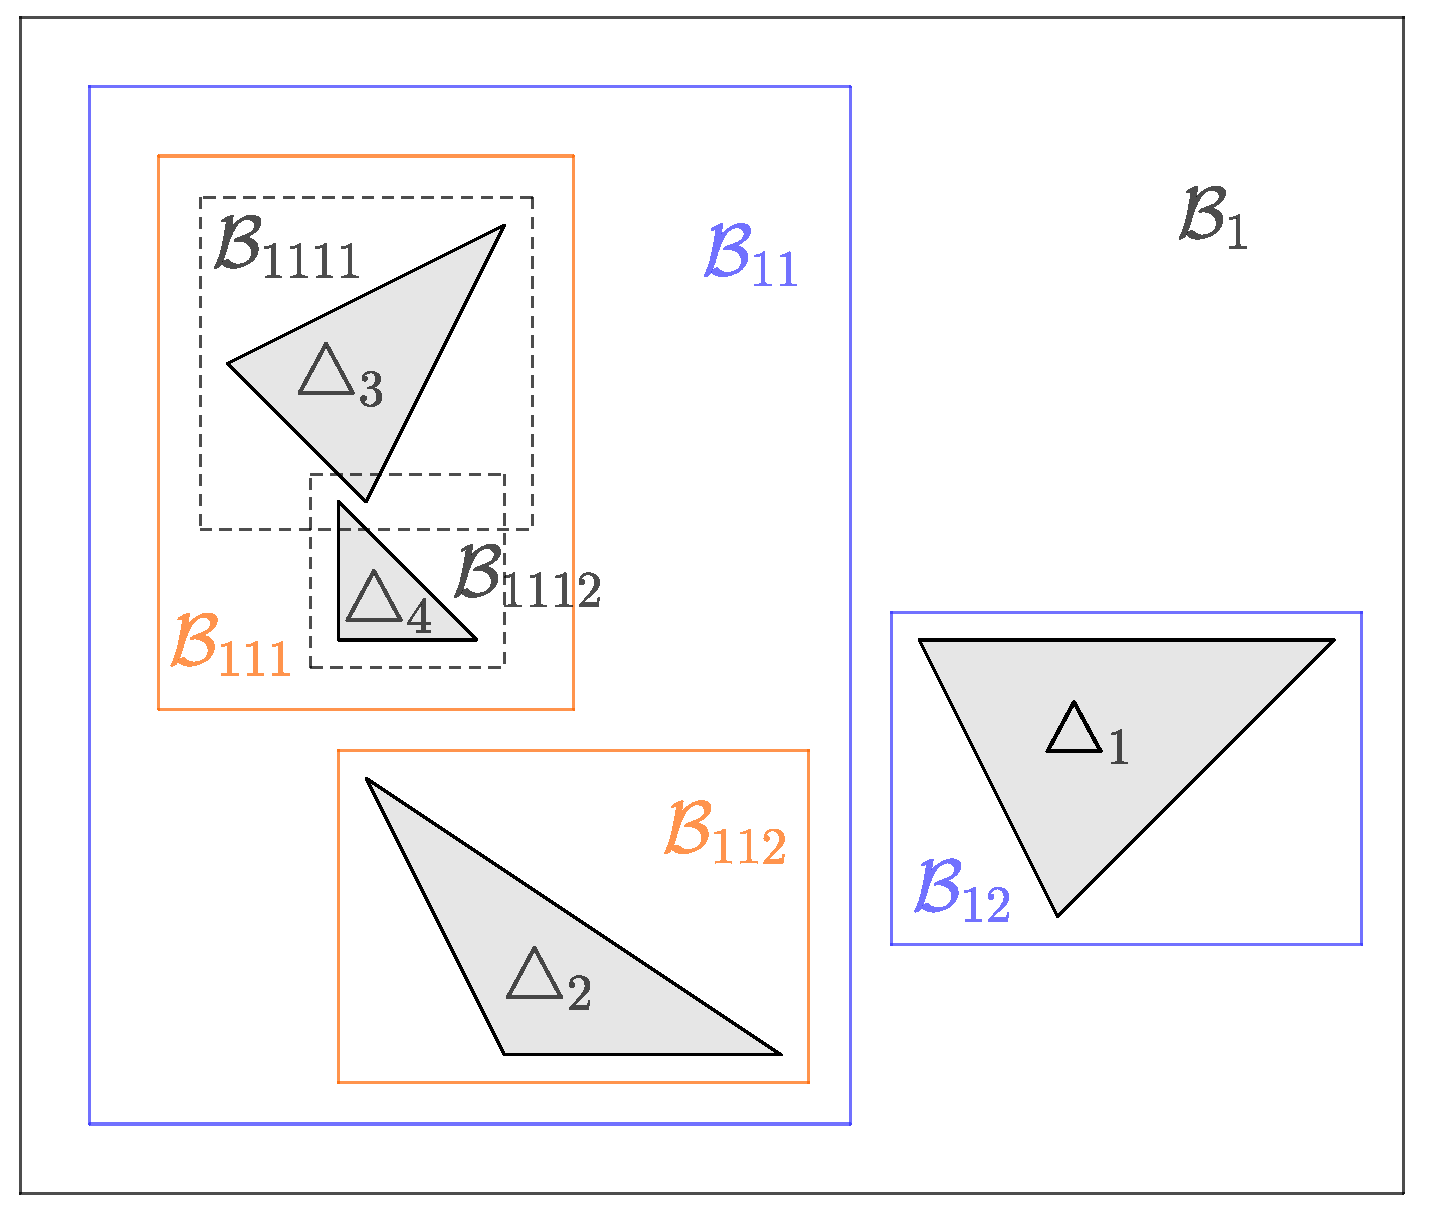
\includegraphics[width=0.95\textwidth]{images/bvh_bounding_boxes.pdf}
        \end{subfigure}
        \begin{subfigure}[b]{0.49\textwidth}
          \center
          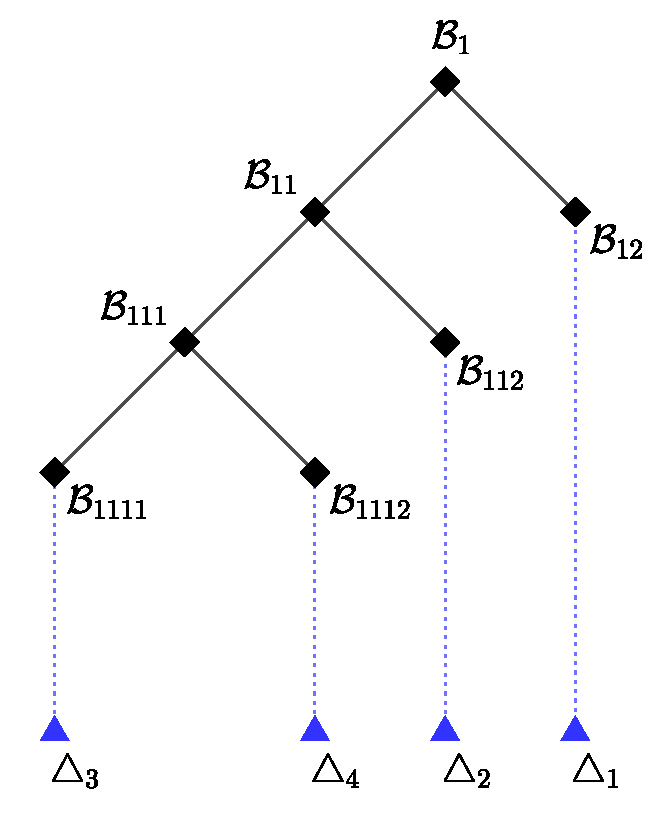
\includegraphics[width=0.75\textwidth]{images/bvh_tree.pdf}
        \end{subfigure}
        \caption{%
          Die Abbildungen zeigen die skizzenhafte Darstellung einer möglichen BVH einer Szene bestehend aus den Dreiecken $\triangle_1$, $\triangle_2$, $\triangle_3$ und $\triangle_4$.
          Im linken Bild sind die \textit{Bounding Boxes} der BVH und im rechten Bild deren zugehörige Verknüpfungen im Sinne eines Baums gezeigt.
        }
        \label{fig:bvh-scheme}
      \end{figure}

      Um die Schnittpunktberechnung zwischen Strahl und \textit{Bounding Box} so weit wie möglich zu vereinfachen, werden an den Koordinatenachsen ausgerichtete \textit{Bounding Boxes} (AABB, engl.: \textit{axis-aligned bounding box}) verwendet.
      Diese lassen sich eindeutig durch die Angabe zweier ihrer gegenüberliegenden Eckpunkte beschreiben.
      Eine AABB beschreibt damit einen Quader im Raum.
      Aus diesem Grund muss für jede der sechs Flächen ein Schnittpunkttest durchgeführt werden.
      Durch die Ausrichtung an den Koordinatenachsen vereinfachen sich diese sechs Tests jedoch zu einer Division, sechs Additionen und sechs Multiplikationen.

      Um BVHs zu konstruieren lassen sich diverse Algorithmen verwenden.
      Im Projekt wählte ich eine Methode, die sowohl auf der CPU als auch GPU effizient funktionieren sollte.
      \textit{Linear Bounding Volume Hierarchies} (LBVH) können in linearer Zeit bezüglich der Anzahl der Dreiecke konstruiert werden.
      Sie sind vergleichsweise einfach parallelisierbar und skalieren sowohl auf der CPU als auch auf der GPU.

      Die Idee besteht darin, die Konstruktion einer LBVH auf ein Sortierverfahren zurückzuführen.
      Da es im dreidimensionalem Raum keine eindeutig ausgezeichnete Ordnung gibt, verwendet man \textit{Morton Codes}.
      Diese bilden naheliegende dreidimensionale Punkte auf naheliegende eindimensionale Punkte entlang einer Kurve ab.
      Aufgrund ihrer charakteristischen Form wird diese Kurve auch die Z-Kurve genannt.
      Abbildung \ref{fig:morton-curve-scheme} zeigt den Verlauf der Morton-Kurve für zwei unterschiedlich feine Gitter.
      Zudem zeigt sie, dass \textit{Morton Codes} auf einer simplen Transformation basieren.
      Gegeben sei für ein $n\in\setNatural$ ein Tupel natürlicher Zahlen $k\in\setNatural_0^n$.
      Die Binärdarstellung einer Koordinate $k_i$ für $i\in\setNatural_0$ mit $i<n$ sei gegeben durch
      \[
        k_i = (\cdots k_{i3}\, k_{i2}\, k_{i1}\, k_{i0})_2
      \]
      In diesem Falle berechnet sich der \textit{Morton Code} $m(k)$ von $k$ durch den folgenden Ausdruck.
      \[
        m(k) \define (\cdots k_{22}\, k_{12}\, k_{02}\cdots k_{21}\, k_{11}\, k_{01}\cdots k_{20}\,k_{10}\,k_{00})_2
      \]
      Durch die Verwendung von \textit{Radix Sort} und der \textit{Morton Codes} der Dreiecksmittelpunkte lässt sich nun durch ein \textit{Bottom-Up}-Verfahren die BVH effizient und parallel konstruieren.
      \begin{figure}[h]
        \center
        \begin{subfigure}[c]{0.49\textwidth}
          \center
          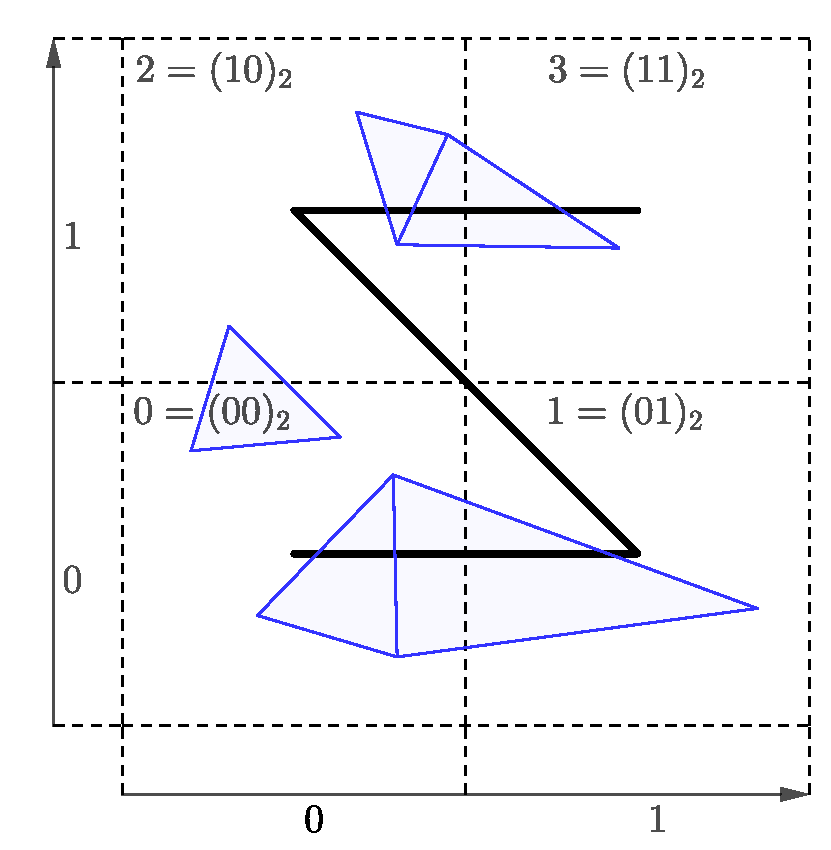
\includegraphics[width=0.95\textwidth]{images/morton_curve_1.pdf}
        \end{subfigure}
        \begin{subfigure}[c]{0.478\textwidth}
          \center
          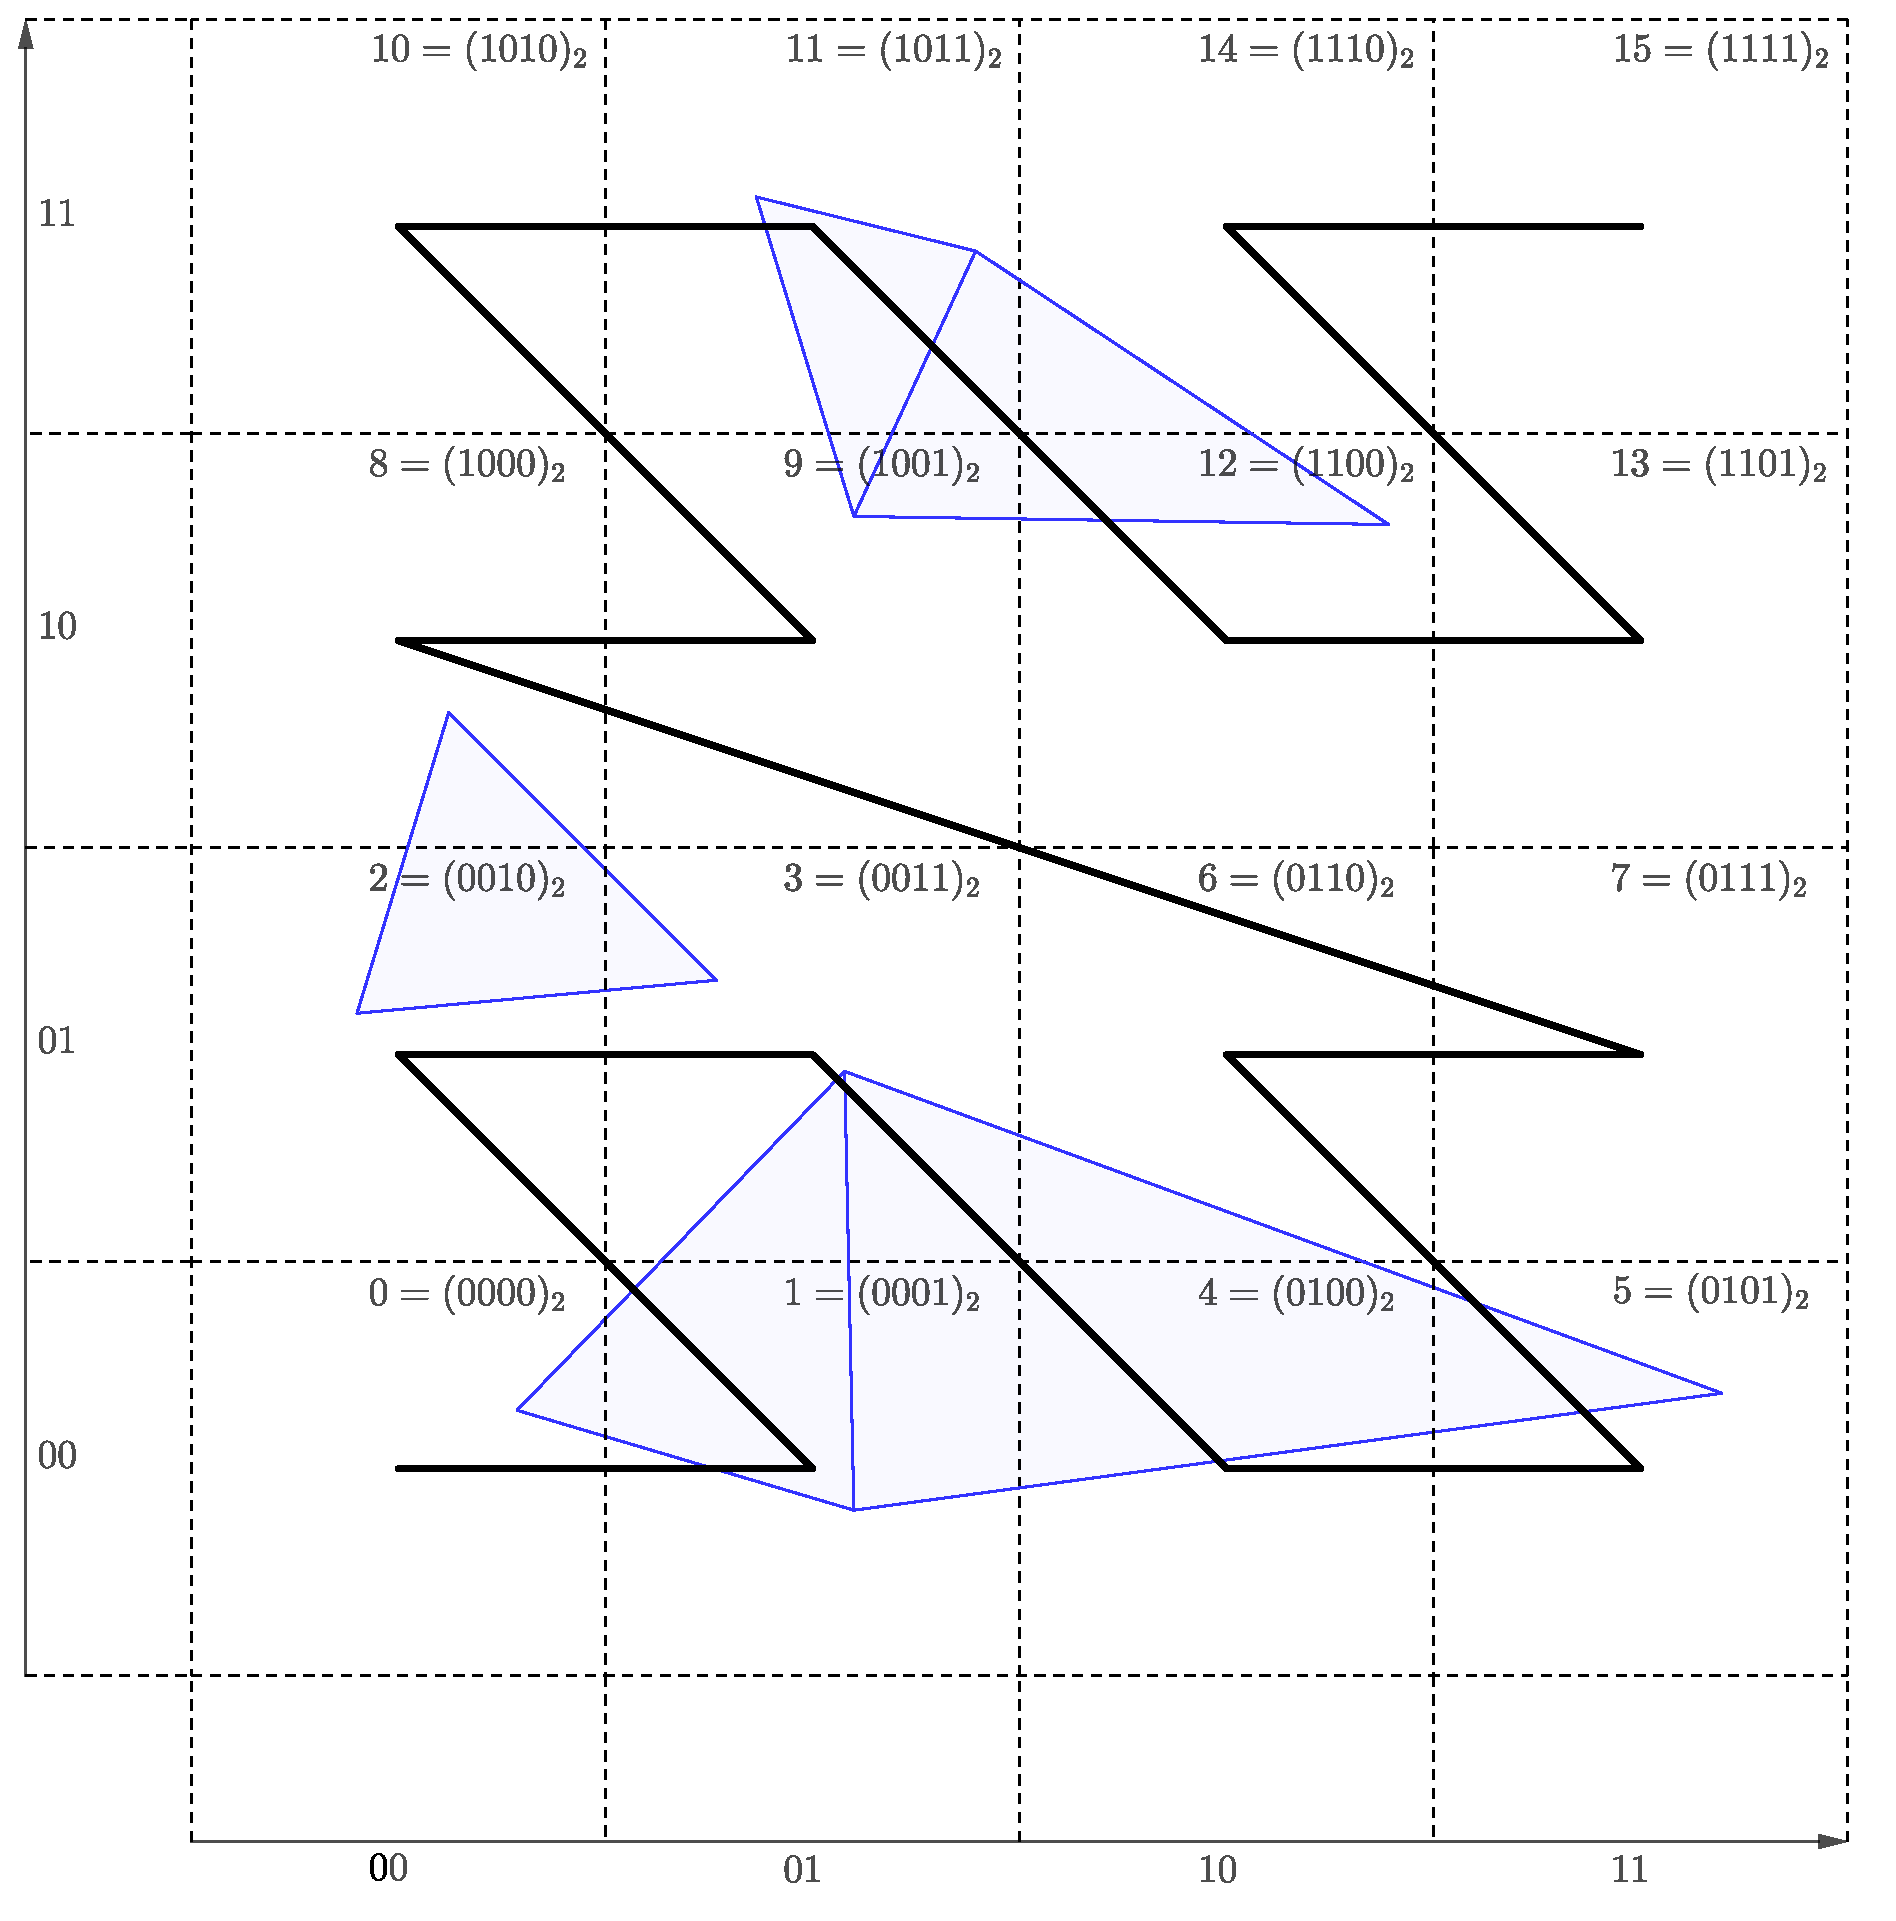
\includegraphics[width=0.95\textwidth]{images/morton_curve_2.pdf}
        \end{subfigure}
        \caption{%
          Die Abbildung zeigt den Verlauf der Morton-Kurve durch die Szene für zwei unterschiedliche Verfeinerungsgrade der Gitter.
        }
        \label{fig:morton-curve-scheme}
      \end{figure}

      Die Struktur einer BVH führt dazu, dass die Laufzeitkomplexität im Durchschnitt logarithmisch statt linear in der Anzahl der Dreiecke verläuft.
      Dies führte zu einer dramatischen Verbesserung der vorherigen Ergebnisse.
      Abbildung \ref{fig:lbvh-results} zeigt vier der im Projekt verwendeten hochkomplexen Modelle.
      Jede Szene konnte durch User-Interaktion mit durchschnittlich $50\appendUnit{FPS}$ rotiert werden.
      Damit übertraf die Verwendung der LBVH jede meiner Erwartungen.
      Auch die Konstruktion der LBVH war innerhalb von ein paar Millisekunden abgeschlossen.
      Doch auch dieser extrem performante Build-Prozess offenbarte nach genaueren Messungen einige Schwachstellen.
      Die entstehende BVH stellt keine optimale BVH der Szene dar.
      Sobald sich die Kamera innerhalb eines Objektes befand, verlangsamte sich das gesamte Rendering.
      Im Verlauf des Projektes wurden innerhalb meiner Arbeitsgruppe weitere Verfahren zur Konstruktion von BVHs eingebaut.
      Es scheint als würden die besten Bäume durch hybride Verwendung von mehreren Methoden entstehen.
      \begin{figure}[h]
        \center
        \begin{subfigure}[b]{0.24\textwidth}
          \center
          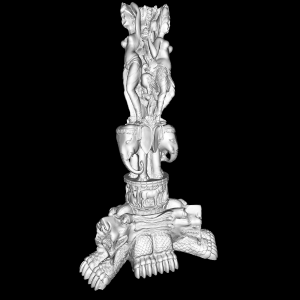
\includegraphics[width=0.95\textwidth]{images/thai_statue.png}
          \caption{\textit{Thai Statue}}
        \end{subfigure}
        \begin{subfigure}[b]{0.24\textwidth}
          \center
          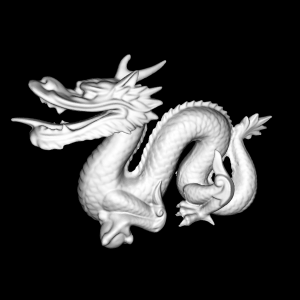
\includegraphics[width=0.95\textwidth]{images/dragon.png}
          \caption{\textit{Chinese Dragon}}
        \end{subfigure}
        \begin{subfigure}[b]{0.24\textwidth}
          \center
          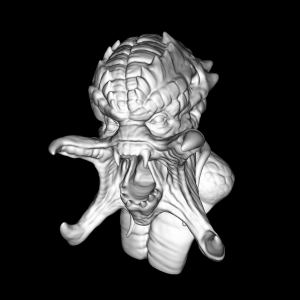
\includegraphics[width=0.95\textwidth]{images/predator.png}
          \caption{\textit{Predator}}
        \end{subfigure}
        \begin{subfigure}[b]{0.24\textwidth}
          \center
          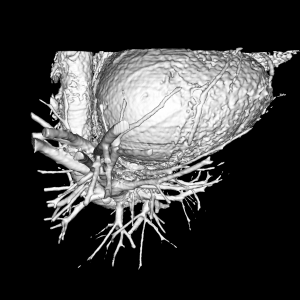
\includegraphics[width=0.95\textwidth]{images/half_heart.png}
          \caption{\textit{Half Heart}}
        \end{subfigure}
        \caption{%
          Die Abbildungen zeigen vier Modell, welche durch den Raytracer gerendert wurden.
          Aufgrund der extrem hohen Dreiecksanzahl war es erst durch die Verwendung einer Beschleunigungsstruktur, wie der LBVH, möglich diese Bilder in Echtzeit zu generieren.
        }
        \label{fig:lbvh-results}
      \end{figure}

    % subsection linear_bounding_volume_hierarchies (end)

    \subsection{Path Tracing} % (fold)
    \label{sub:path_tracing}
      \subsubsection{Quasi-Monte-Carlo-Methoden} % (fold)
      \label{ssub:monte_carlo_methoden}

      % subsubsection monte_carlo_methoden (end)

      \subsubsection{Light Caching} % (fold)
      \label{ssub:light_caching}

      % subsubsection light_caching (end)

      \subsubsection{Reflexions- und Brechungsmodelle} % (fold)
      \label{ssub:reflexions_und_brechungsmodelle}

      % subsubsection reflexions_und_brechungsmodelle (end)
    % subsection path_tracing (end)

    \subsection{Optimierungen auf CPU} % (fold)
    \label{sub:optimierungen_auf_cpu}
      \subsubsection{Threadpools, OpenMP, mctp} % (fold)
      \label{ssub:threadpools}

      % subsubsection threadpools (end)

      \subsubsection{SIMD intrinsics} % (fold)
      \label{ssub:simd_intrinsics}

      % subsubsection simd_intrinsics (end)
    % subsection optimierungen_auf_cpu (end)

    \subsection{Übertragung auf die GPU} % (fold)
    \label{sub:uebertragung_auf_die_gpu}
      Funktionsweise GPU, textures, CUDA, SIMD
    % subsection übertragung_auf_die_gpu (end)
  % section beschleunigungsstrukturen_optimierung_und_weitere_features (end)
\end{document}